\documentclass{article}
\usepackage{graphicx} % Required for inserting images
\usepackage{enumitem}
\usepackage{xcolor}
\usepackage{listings}
\usepackage{mathtools}
\usepackage{amsmath}
\newcommand{\logicarg}[2]{% \logicarg{<premise>}{<conclusion>}
  \begin{tabular}[t]{@{}l@{}}
    #1 \\ \hline #2
  \end{tabular}%
}

\setlength{\oddsidemargin}{-0.25in}
\setlength{\topmargin}{-0.5in}
\setlength{\headheight}{0cm}
\setlength{\headsep}{0cm}
\setlength{\textheight}{10in}
\setlength{\textwidth}{7in}
\setlength{\topskip}{0cm}

\begin{document}

\noindent\textbf{ComS 472 - PS6 \quad Due: Oct 27, 2024 \quad Name: Aren Ashlock}

\begin{enumerate}

% ------------------------------------- 1 DONE -------------------------------------

\item \textbf{(12 pts)} (Exercise 6.1) Which of the following are correct? No explanation is needed. The operator $\models$ always has the lowest precedence.

    \begin{enumerate}[label=($\alph*$)]

    % ----------------------------------- 1a DONE -----------------------------------

    \item False $\models$ True.

    \color{blue}
        Correct
    \color{black}

    % -------------------------------------------------------------------------------

    % ----------------------------------- 1b DONE -----------------------------------

    \item True $\models$ False.

    \color{blue}
        Incorrect
    \color{black}

    % -------------------------------------------------------------------------------

    % ----------------------------------- 1c DONE -----------------------------------

    \item $A \wedge B \models A \Leftrightarrow B$.

    \color{blue}
        Correct
    \color{black}

    % -------------------------------------------------------------------------------

    % ----------------------------------- 1d DONE -----------------------------------

    \item $A \Leftrightarrow B \models A \vee B$.

    \color{blue}
        Incorrect
    \color{black}

    % -------------------------------------------------------------------------------

    % ----------------------------------- 1e DONE -----------------------------------

    \item $A \Leftrightarrow B \models \neg A \vee B$.

    \color{blue}
        Correct
    \color{black}

    % -------------------------------------------------------------------------------

    % ----------------------------------- 1f DONE -----------------------------------

    \item $(A \vee B) \wedge (\neg C \vee \neg D \vee E) \models (A \vee B \vee C) \wedge (B \wedge C \wedge D \Rightarrow E)$.

    \color{blue}
        Correct
    \color{black}

    % -------------------------------------------------------------------------------

    % ----------------------------------- 1g DONE -----------------------------------

    \item $(A \vee B) \wedge (\neg C \vee \neg D \vee E) \models (A \vee B) \wedge (\neg D \vee E)$.

    \color{blue}
        Incorrect
    \color{black}

    % -------------------------------------------------------------------------------

    % ----------------------------------- 1h DONE -----------------------------------

    \item $(A \vee B) \wedge \neg (A \Rightarrow B)$ is satisfiable.

    \color{blue}
        Correct
    \color{black}

    % -------------------------------------------------------------------------------

    % ----------------------------------- 1i DONE -----------------------------------

    \item $(A \wedge B) \Rightarrow C \models (A \Rightarrow C) \vee (B \Rightarrow C)$.

    \color{blue}
        Correct
    \color{black}

    % -------------------------------------------------------------------------------

    % ----------------------------------- 1j DONE -----------------------------------

    \item $(C \vee (\neg A \wedge \neg B)) \equiv ((A \Rightarrow C) \wedge (B \Rightarrow C))$

    \color{blue}
        Correct
    \color{black}

    % -------------------------------------------------------------------------------

    % ----------------------------------- 1k DONE -----------------------------------

    \item $(A \Leftrightarrow B) \wedge (\neg A \vee B)$ is satisfiable.

    \color{blue}
        Correct
    \color{black}

    % -------------------------------------------------------------------------------

    % ----------------------------------- 1l DONE -----------------------------------

    \item $(A \Leftrightarrow B) \Leftrightarrow C$ has the same number of models as $A \Leftrightarrow B$ for any fixed set of proposition symbols that includes $A, B, C$.

    \color{blue}
        Incorrect
    \color{black}

    % -------------------------------------------------------------------------------
    
    \end{enumerate}

% ----------------------------------------------------------------------------------

% ------------------------------------- 2 DONE -------------------------------------

\item \textbf{(9 pts)} (Exercise 7.7) Prove, or find a counterexample to, each of the following assertions:

    \begin{enumerate}[label=($\alph*$)]

    % ----------------------------------- 2a DONE -----------------------------------

    \item \textbf{(3 pts)} If $\alpha \models \gamma$ or $\beta \models \gamma$ (or both) then $\alpha \wedge \beta \models \gamma$.

    \color{blue}
        This assertion is \textbf{true}. There are 2 cases that need to be proved:\\
        \textbf{1.} When both $\alpha \models \gamma$ and $\beta \models \gamma$, which means that both $\alpha$ and $\beta$ are subsets of $\gamma$. In this case, if there is any intersection between $\alpha$ and $\beta$, then that itself is a subset of $\gamma$ since both sets are encompassed by $\gamma$ meaning any shared models are encompassed by $\gamma$ as well. This means the assertion is true for this situation.\\
        \textbf{2.} When either $\alpha \models \gamma$ or $\beta \models \gamma$, which means that whichever set of models entails $\gamma$ is a subset of $\gamma$. In this case, we know one of the sets of models (either $\alpha$ or $\beta$) is entirely encompassed by $\gamma$. Therefore, any intersection between $\alpha$ and $\beta$ will lie within $\gamma$ making it a subset. This means the assertion is true in either of those situations.
    \color{black}

    % -------------------------------------------------------------------------------

    % ----------------------------------- 2b DONE -----------------------------------

    \item \textbf{(3 pts)} If $\alpha \wedge \beta \models \gamma$ then $\alpha \models \gamma$ or $\beta \models \gamma$ (or both).

    \color{blue}
        This assertion is \textbf{false}. An example of this can be the following: $M(\alpha)$ is $x \geq 0$, $M(\beta)$ is $x \leq 0$, and $M(\gamma)$ is $x = 0$.\\
        In this circumstance, when $\alpha \wedge \beta$ is true, it's only for $x = 0$ which is a subset of $M(\gamma)$. However, there are values in $M(\alpha)$ and $M(\beta)$ (independent of each other) that are not found within $M(\gamma)$. Therefore, $\alpha \models \gamma$ and $\beta \models \gamma$ are both FALSE, but $\alpha \wedge \beta \models \gamma$ is TRUE. This results in $T \Rightarrow F \vee F$, which is FALSE.
    \color{black}

    % -------------------------------------------------------------------------------

    % ----------------------------------- 2c DONE -----------------------------------

    \item \textbf{(3 pts)} If $\alpha \models (\beta \vee \gamma)$ then $\alpha \models \beta$ or $\alpha \models \gamma$ (or both).

    \color{blue}
        This assertion is \textbf{false}. Here is an example of a possible scenario where $\alpha \models (\beta \vee \gamma)$ is true:\\
        \begin{center}
            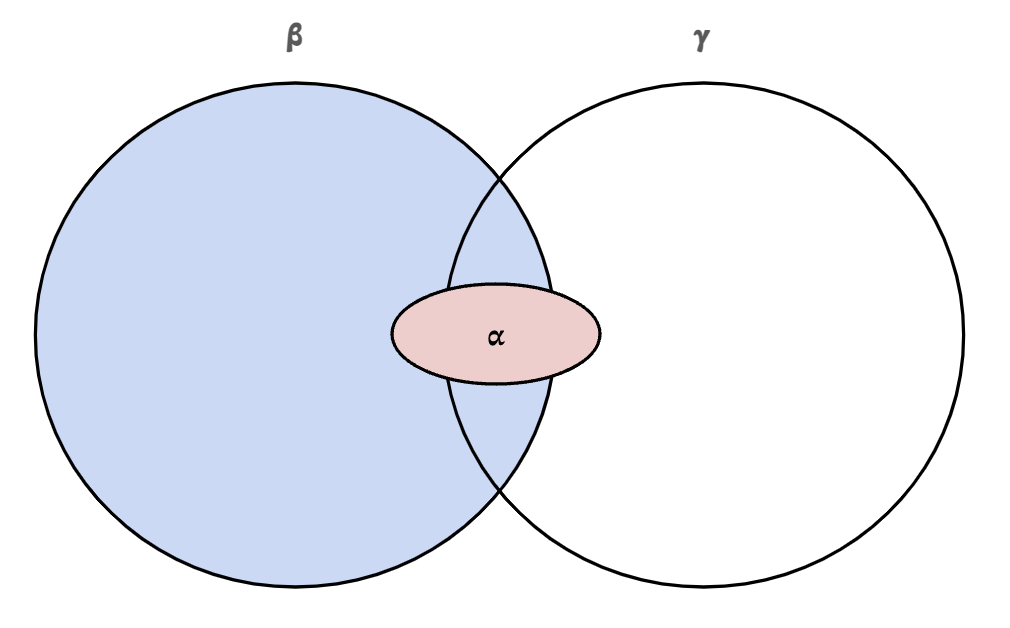
\includegraphics[scale=0.5]{COMS472-PS6-Q2-C.png}
        \end{center}
        As shown by the diagram, it is possible for a model of $\alpha$ to not be in the models of $\beta$ or for a model of $\alpha$ to not be in the models of $\gamma$. Therefore, $\alpha \models \beta$ or $\alpha \models \gamma$ (or both) is false in this instance, thus proving that the assertion is false.
    \color{black}

    % -------------------------------------------------------------------------------
    
    \end{enumerate}

% ----------------------------------------------------------------------------------

% ------------------------------------- 3 DONE -------------------------------------

\item \textbf{(10 pts)} (Exercise 7.16) This exercise looks into the relationship between clauses and implication sentences.

    \begin{enumerate}[label=($\alph*$)]

    % ----------------------------------- 3a DONE -----------------------------------

    \item \textbf{(3 pts)} Show that the clause $\neg P \vee ... \vee \neg P_m \vee Q$ is logically equivalent to the implication sentence $P_1 \wedge ... \wedge P_m \Rightarrow Q$.

    \color{blue}
        The implication sentence is true for all cases other than $T \Rightarrow F$. That will happen when $P_1 \wedge ... \wedge P_m$ is true (so each $P$ must be true) and $Q$ is false. Looking at the clause, that will result in FALSE as well since all $P$ being true will result in false and $Q$ is false.\\\\
        The other instance where $Q$ is false is when at least one of the $P$ is false. In this case, the implication results in $F \Rightarrow F$, which is TRUE. And the clause is true since the negation of at least one $P$ that is false will make it TRUE.\\\\
        Now, if all $P$ are false and $Q$ is true, then the implication results in $F \Rightarrow T$, which is also TRUE. And since $Q$ is true, that means the clause is TRUE.\\\\
        Finally, the only other result of the implication is $T \Rightarrow T$, which happens when $P_1 \wedge ... \wedge P_m$ is true (so each $P$ must be true) and $Q$ is true. Even though $\neg P \vee ... \vee \neg P_m$ will result in false, $Q$ is true, so the clause is TRUE.
    \color{black}

    % -------------------------------------------------------------------------------

    % ----------------------------------- 3b DONE -----------------------------------

    \item \textbf{(4 pts)} Show that every clause (regardless of the number of positive literals) can be written in the form $P_1 \wedge ... \wedge P_m \Rightarrow Q_1 \vee ... \vee Q_n$, where the $P_i$s and $Q_j$s are propositional symbols. (A knowledge base consisting of such sentences is in implicative normal form or Kowalski form.)

    \color{blue}
        1. We know that every clause is written as literals connected using disjunctions.\\
        2. Then, you are able to group the positive and negative literals together with parenthesis since the disjunction symbol has the lowest precedence in a clause. This gives a rough form of $(\neg P_1 \vee ... \vee \neg P_m) \vee (Q_1 \vee ... \vee Q_n)$ where $P$ are the negative literals and $Q$ are the positive literals.\\
        3. Next, apply De Morgan's Law to the $P$ terms to get $\neg ( P_1 \wedge ... \wedge P_m) \vee (Q_1 \vee ... \vee Q_n)$.\\
        4. Finally, you can reverse the "implication elimination" rule ($\neg \alpha \vee \beta$ becomes $\alpha \Rightarrow \beta$) to get $P_1 \wedge ... \wedge P_m \Rightarrow Q_1 \vee ... \vee Q_n$.
    \color{black}

    % -------------------------------------------------------------------------------

    % ----------------------------------- 3c DONE -----------------------------------

    \item \textbf{(3 pts)} Write down the full resolution rule for sentences in implicative normal form.

    \color{blue}
        \logicarg{$a_1 \wedge ... \wedge a_m \Rightarrow b_1 \vee ... \vee b_i \vee ... \vee b_n$ \quad $c_1 \wedge ... \wedge c_j \wedge ... \wedge c_p \Rightarrow d_1 \vee ... \vee d_q$ \quad $b_i, c_j$ and complements}
        {$a_1 \wedge ... \wedge a_m \wedge c_1 \wedge ... \wedge c_{j-1} \wedge c_{j+1} \wedge ... \wedge c_p \Rightarrow b_1 \vee ... \vee b_{i-1} \vee b_{i+1} \vee ... \vee b_n \vee d_1 \vee ... \vee d_q$}
    \color{black}

    % -------------------------------------------------------------------------------
    
    \end{enumerate}

% ----------------------------------------------------------------------------------

% ------------------------------------- 4 DONE -------------------------------------

\item \textbf{(14 pts)} (Exercise 7.21) A propositional 2-CNF expression is a conjunction of clauses, each containing exactly two literals, e.g.,
\begin{gather*}
    (A \vee B) \wedge (\neg A \vee C) \wedge (\neg B \vee D) \wedge (\neg C \vee G) \wedge (\neg D \vee G).
\end{gather*}

    \begin{enumerate}[label=($\alph*$)]

    % ----------------------------------- 4a DONE -----------------------------------

    \item \textbf{(3 pts)} Prove using resolution that the above sentence entails $G$.

    \color{blue}
        $(A \vee B) \wedge (\neg A \vee C) \wedge (\neg B \vee D) \wedge (\neg C \vee G) \wedge (\neg D \vee G)$\\
        $(B \vee C) \wedge (\neg B \vee D) \wedge (\neg C \vee G) \wedge (\neg D \vee G)$\\
        $(B \vee C) \wedge (\neg B \vee G) \wedge (\neg C \vee G)$\\
        $(G \vee C) \wedge (\neg C \vee G)$\\
        $G \vee G$\\
        $G$
    \color{black}

    % -------------------------------------------------------------------------------

    % ----------------------------------- 4b DONE -----------------------------------

    \item \textbf{(4 pts)} Two clauses are \textit{semantically distinct} if they are not logically equivalent. How many semantically distinct 2-CNF clauses can be constructed from $n$ proposition symbols?

    \color{blue}
        Choosing the clauses: $\binom n2=\frac{n(n-1)}{2}$\\
        Since there are 4 ways of arranging positive and negative, we get: $4 \times \frac{n(n-1)}{2}$\\
        \textbf{Answer}: $2n^2-2n$
    \color{black}

    % -------------------------------------------------------------------------------

    % ----------------------------------- 4c DONE -----------------------------------

    \item \textbf{(3 pts)} Using your answer to (b), prove that propositional resolution always terminates in time polynomial in $n$, given a 2-CNF sentence containing no more than n distinct symbols.

    \color{blue}
        From (b), we know there are at most $2n^2-2n$ distinct 2-CNF clauses, so there can be a maximum of that many clauses in a propositional expression. The worst resolution can perform is going from the maximum number of clauses to a single clause, which will perform $2n^2-2n-1$ resolutions since each resolution step can only reduce one at a time and the result will always be at most another 2-CNF. Thus, looking at the big-O notation, it will terminate in $O(n^2)$.
    \color{black}

    % -------------------------------------------------------------------------------

    % ----------------------------------- 4d DONE -----------------------------------

    \item \textbf{(4 pts)} Explain why your argument in (c) does not apply to 3-CNF.

    \color{blue}
        With 2-CNF, resolution will make 2 clauses resolve into another 2-CNF clause. However, with 3-CNF, resolution will make it a 4-CNF, which can continue to grow with further resolutions. Therefore, we cannot know that resolution will terminate in polynomial time
    \color{black}

    % -------------------------------------------------------------------------------
    
    \end{enumerate}

% ----------------------------------------------------------------------------------

% ------------------------------------- 5 DONE -------------------------------------

\item \textbf{(15 pts)} (Exercise 7.23) Consider the following sentence:
\begin{gather*}
    ((\text{Food} \Rightarrow \text{Party}) \vee (\text{Drinks} \Rightarrow \text{Party})) \Rightarrow ((\text{Food} \wedge \text{Drinks}) \Rightarrow \text{Party}).
\end{gather*}

    \begin{enumerate}[label=($\alph*$)]

    % ----------------------------------- 5a DONE -----------------------------------

    \item \textbf{(5 pts)} Determine, using enumeration, whether this sentence is valid, satisfiable (but not valid), or unsatisfiable.

    \color{blue}
        (I'm using $F$ as Food, $D$ as Drinks, and $P$ as Party in the header. In the table, $T$ and $F$ still mean True and False)
        \begin{displaymath}
        \begin{array}{|c c c|c c c c c|c|}
            F & D & P & (F \Rightarrow P) & (D \Rightarrow P) & ((F \Rightarrow P) \vee (D \Rightarrow P)) & (F \wedge D) & ((F \wedge D) \Rightarrow P) & \text{Result}\\
            \hline
            T & T & T & T & T & T & T & T & T\\
            T & T & F & F & F & F & T & F & T\\
            T & F & T & T & T & T & F & T & T\\
            T & F & F & F & T & T & F & T & T\\
            F & T & T & T & T & T & F & T & T\\
            F & T & F & T & F & T & F & T & T\\
            F & F & T & T & T & T & F & T & T\\
            F & F & F & T & T & T & F & T & T
        \end{array}
        \end{displaymath}

        Based on the enumeration, the sentence is \textbf{valid}.
    \color{black}

    % -------------------------------------------------------------------------------

    % ----------------------------------- 5b DONE -----------------------------------

    \item \textbf{(5 pts)} Convert the left-hand and right-hand sides of the main implication into CNF, showing each step, and explain how the results confirm your answer to (a).

    \color{blue}
        \textbf{Start:} $((\text{Food} \Rightarrow \text{Party}) \vee (\text{Drinks} \Rightarrow \text{Party})) \Rightarrow ((\text{Food} \wedge \text{Drinks}) \Rightarrow \text{Party})$\\
        $((\neg \text{Food} \vee \text{Party}) \vee (\text{Drinks} \Rightarrow \text{Party})) \Rightarrow ((\text{Food} \wedge \text{Drinks}) \Rightarrow \text{Party})$ \quad [implication elimination]\\
        $((\neg \text{Food} \vee \text{Party}) \vee (\neg \text{Drinks} \vee \text{Party})) \Rightarrow ((\text{Food} \wedge \text{Drinks}) \Rightarrow \text{Party})$  \quad [implication elimination]\\
        $(\neg \text{Food} \vee \text{Party} \vee \neg \text{Drinks} \vee \text{Party}) \Rightarrow ((\text{Food} \wedge \text{Drinks}) \Rightarrow \text{Party})$  \quad [drop unnecessary ()]\\
        $(\neg \text{Food} \vee \neg \text{Drinks} \vee \text{Party} \vee \text{Party}) \Rightarrow ((\text{Food} \wedge \text{Drinks}) \Rightarrow \text{Party})$  \quad [commutativity of $\vee$]\\
        $(\neg \text{Food} \vee \neg \text{Drinks} \vee \text{Party}) \Rightarrow ((\text{Food} \wedge \text{Drinks}) \Rightarrow \text{Party})$  \quad [Party $\vee$ Party $\equiv$ Party]\\
        $(\neg \text{Food} \vee \neg \text{Drinks} \vee \text{Party}) \Rightarrow (\neg (\text{Food} \wedge \text{Drinks}) \vee \text{Party})$  \quad [implication elimination]\\
        $(\neg \text{Food} \vee \neg \text{Drinks} \vee \text{Party}) \Rightarrow ((\neg \text{Food} \vee \neg \text{Drinks}) \vee \text{Party})$  \quad [De Morgan]\\
        $(\neg \text{Food} \vee \neg \text{Drinks} \vee \text{Party}) \Rightarrow (\neg \text{Food} \vee \neg \text{Drinks} \vee \text{Party})$  \quad [drop unnecessary ()]\\
        
        \textbf{Explanation:} As shown, the left-hand and right-hand sides are equivalent. Therefore, the main implication can only result in $T \Rightarrow T$ or $F \Rightarrow F$, which both are TRUE. This shows how in every model, the sentence is true, which is the definition of \textbf{valid}.
    \color{black}

    % -------------------------------------------------------------------------------

    % ----------------------------------- 5c DONE -----------------------------------

    \item \textbf{(5 pts)} Prove your answer to (a) using resolution.

    \color{blue}
        To prove it, we have our KB on conjuctions, which is the left-hand side. We add $\neg \alpha$, the right-hand side. Then show it results in an empty clause after resolution. (I'm going to start with the final form from 5b...)\\
        KB: (1) $(\neg \text{Food} \vee \neg \text{Drinks} \vee \text{Party})$\\
        $\neg \alpha$: $(\text{Food} \wedge \text{Drinks} \wedge \neg \text{Party})$ \quad [Add each conjunction to the KB]\\
        KB: (1) $(\neg \text{Food} \vee \neg \text{Drinks} \vee \text{Party})$, (2) Food, (3) Drinks, (4) $\neg$ Party\\
        1. (1) $(\neg \text{Food} \vee \neg \text{Drinks} \vee \text{Party})$ and (2) Food results in (5) $(\neg \text{Drinks} \vee \text{Party})$\\
        2. (5) $(\neg \text{Drinks} \vee \text{Party})$ and (3) Drinks results in (6) Party\\
        3. (6) Party and (4) $\neg$ Party results in an empty clause.\\
        \textbf{Therefore,} there must be a contradiction meaning the original sentence must be valid. This backs up my answer to (a).
    \color{black}

    % -------------------------------------------------------------------------------
    
    \end{enumerate}

% ----------------------------------------------------------------------------------

\end{enumerate}
\end{document}